\section{Introduction}

Asynchronous audio communication (AAC) is rapidly becoming available to mass audiences through social platforms such as WhatsApp, iMessage, and Facebook. 
While text is still by far the most prevalent mode of communication on the Internet, audio is desirable in many situations because it allows users to deliver more expressive, nuanced messages than text.
AAC also holds considerable potential for improving online education, where voice communication has been shown to improve student-student and student-instructor engagement as well as a sense of the instructor's social presence \cite{ice,oomen,tu}. 

The problem with replacing textual communication with speech, however, is that speakers may face difficulty articulating their ideas vocally.
For instance, a 2002 study using Wimba voice boards for discussion forums found that students overwhelmingly preferred text over speech comments, in part because it required them to speak fluently without making errors \cite{wimba}.
Since this problem affects students even in physical classrooms, it could certainly prevent some learners from participating in online oral discussions.
AAC platforms in such situations, then, must somehow compensate for the linearity and immutability of audio on the production side.

\begin{figure}
	\centering
	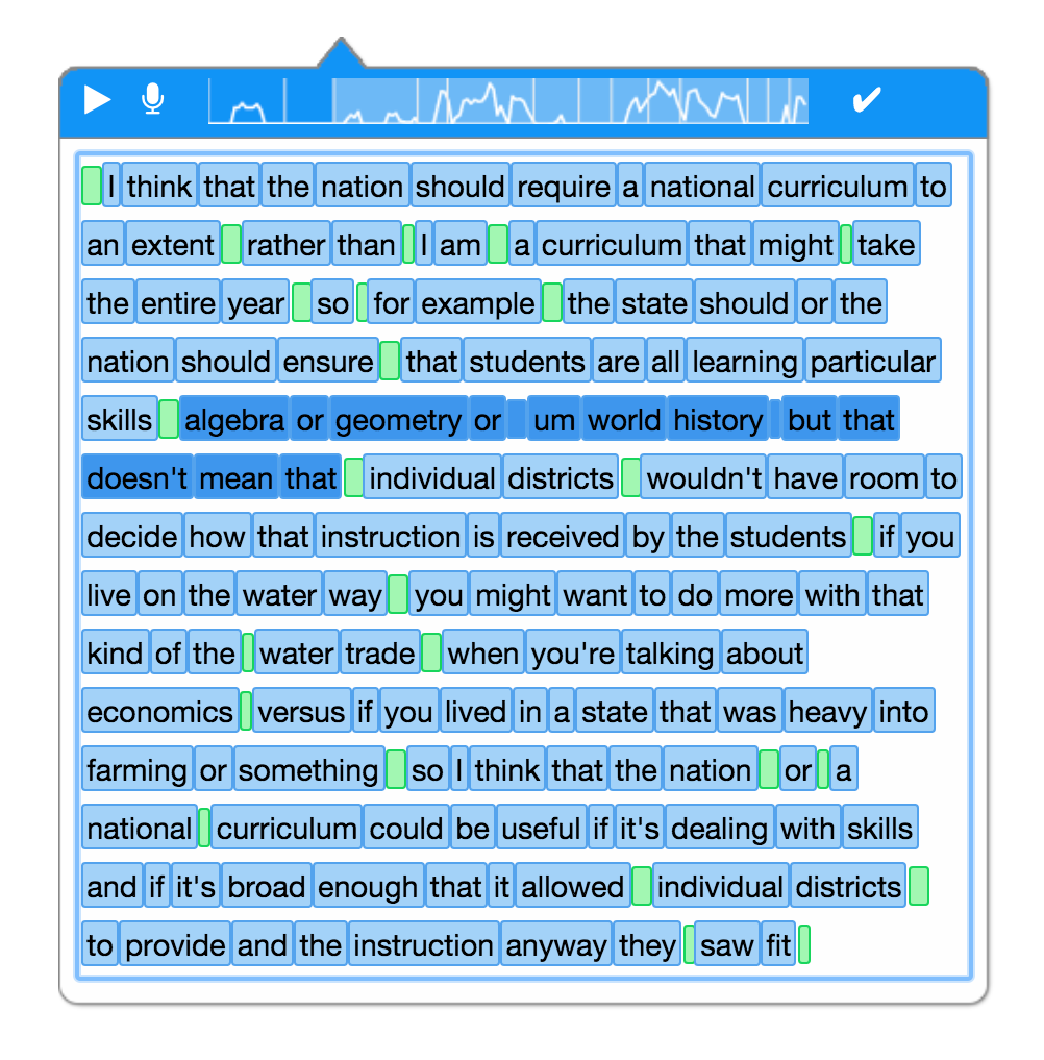
\includegraphics[width=\columnwidth,keepaspectratio]{figures/large_screenshot}
	\caption{The user interface for SimpleSpeech presents an automatically-generated transcription of a voice comment, which can then be manipulated through normal word-processing operations, such as selection, deletion, and insertion. Word and pause tokens are mapped with audio via time alignment data.ß}~\label{fig:overview_shot}
\end{figure}

Our solution is to provide lightweight, easy-to-use editing tools based on automatic speech recognition (ASR)-generated transcripts.
Many prior studies have utilized transcription to assist in audio editing \cite{casares,rubin,whittaker_semantic}, but only recently has fast, live editing become possible through advances in ASR technology \cite{baker,saon}.
We designed and developed an audio production tool, which we call SimpleSpeech, that allows users to delete and insert segments of the recording in real-time by manipulating a tokenized text representation. 
Our user interface design focuses primarily on simplifying quick word-level editing and visually reinforcing the mapping between the source audio and the text, which helps users edit when transcription errors are present.

Qualitative evidence indicates that SimpleSpeech's simplified interface gave users enough control over the editing process and enabled them to produce more polished audio comments in an online forum discussion.
A subsequent quantitative evaluation with high school students showed that the mental workload of recording voice messages was significantly decreased with editing functionality, demonstrating that SimpleSpeech would be a valuable enhancement to online audio communication platforms.
Finally, some linguistic characteristics of messages created using AAC are also discussed in comparison to other forms of communication, leading to new considerations and insights on optimal applications of this technology.